\documentclass[unicode]{beamer}

\usepackage[utf8]{inputenc}
\usepackage{cmap}
\usepackage[russian]{babel}

% listings
\usepackage{listings}
\lstset{language=java,frame=shadowbox,rulesepcolor=\color{gray},
        resetmargins=true,showstringspaces=false,
        basicstyle=\ttfamily,keywordstyle=\color{blue},
        stringstyle=\color{purple},commentstyle=\color{gray},
        morekeywords={assert,enum,@interface}}

% beamer
\usetheme{CambridgeUS}

\beamertemplatenavigationsymbolsempty

\setbeamertemplate{bibliography item}[book]
\setbeamertemplate{bibliography entry note}{//~}
\setbeamercolor{bibliography entry note}{fg=structure}

\title[Разработка сетевых приложений]{Разработка сетевых приложений на Java}
\author{Алексей Владыкин}
\date{27 ноября 2017}

\begin{document}

\begin{frame}
\titlepage
\end{frame}

\begin{frame}
\tableofcontents
\end{frame}


\section{Как компьютеры общаются между собой?}

\begin{frame}
\begin{columns}
\begin{column}{0.6\textwidth}
Стек протоколов:
\begin{itemize}
\item Прикладной уровень\\(HTTP, FTP, SSH, \ldots)
\item Транспортный уровень\\(TCP, UDP, \ldots)
\item Сетевой уровень
\item Канальный уровень
\end{itemize}
\end{column}%
\begin{column}{0.4\textwidth}
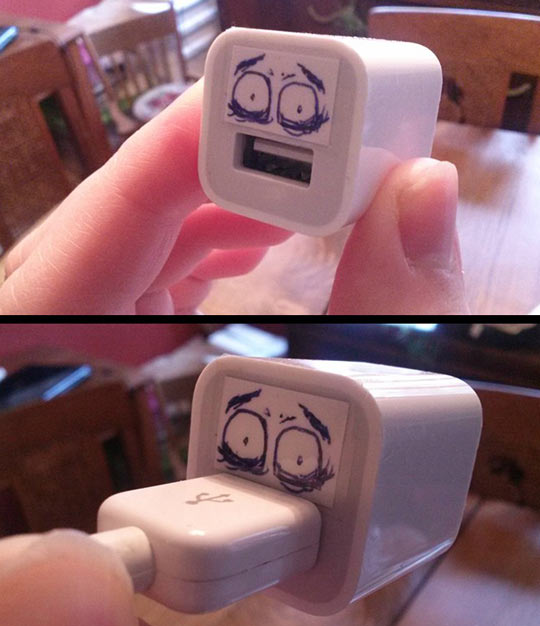
\includegraphics[width=0.9\textwidth]{pics/socket.jpg}
\end{column}
\end{columns}
\end{frame}


\begin{frame}{TCP}
\begin{itemize}
\item \structure{Transmission Control Protocol}
\bigskip
\item Протокол транспортного уровня
\item С установлением соединения
\item С гарантиями доставки и порядка
\end{itemize}
\end{frame}


\begin{frame}{UDP}
\begin{itemize}
\item \structure{User Datagram Protocol}
\bigskip
\item Протокол транспортного уровня
\item Без установления соединения
\item Без гарантий доставки и порядка
\item Но зато минимизируются задержки
\end{itemize}
\end{frame}


\begin{frame}[fragile]{HTTP}
\textbf{Request:}
\begin{verbatim}
GET / HTTP/1.1
Host: localhost
User-Agent: Mozilla/5.0 (Windows NT 6.3; WOW64; rv:50.0)
  Gecko/20100101 Firefox/50.0
\end{verbatim}
\bigskip
\textbf{Response:}
\begin{verbatim}
HTTP/1.1 200 OK
Content-Type: text/html

<h1>Hello world</h1>
\end{verbatim}
\end{frame}


\begin{frame}{Поддержка в Java}
\begin{itemize}
\item TCP:\\
java.net.Socket и java.net.ServerSocket
\bigskip
\item UDP:\\
java.net.DatagramSocket
\bigskip
\item HTTP:\\
java.net.URL (но лучше сторонние библиотеки)\\
в Java 9 --- экспериментальный HTTP/2 клиент \texttt{jdk.incubator.httpclient}
\end{itemize}
\end{frame}


\section{Пишем свой HTTP-сервер}

\begin{frame}{HTTP-сервер на <<голых>> сокетах}
\begin{itemize}
\item Демо
\bigskip
\item Ручной разбор заголовков
\item Отдельный Thread на каждого клиента – организуем вручную
\end{itemize}
\end{frame}


\begin{frame}{HTTP-сервер на Netty}
\begin{itemize}
\item Демо
\bigskip
\item Особенности протокола HTTP и многопоточность скрыты Netty
\item Пишем только бизнес-логику
\end{itemize}
\end{frame}


\begin{frame}{Сервлеты}
\begin{itemize}
\item Сервлет --- Java-класс, унаследованный от javax.servlet.http.HttpServlet
\bigskip
\item Работает под управлением контейнера сервлетов (IoC)\\
Tomcat, Jetty, \ldots
\bigskip
\item Часть Java Enterprise Edition
\bigskip
\item Демо
\end{itemize}
\end{frame}


\begin{frame}{Сервлеты}
\begin{itemize}
\item Требуется конфигурационный файл WEB-INF/web.xml
\item Либо аннотация @WebServlet (если контейнер поддерживает Servlet 3.0)
\end{itemize}
\end{frame}


\begin{frame}{Сервлеты}
\begin{itemize}
\item Особенности HTTP и организацию многопоточности берет на себя контейнер сервлетов
\item Поддержка пользовательской сессии
\bigskip
\item В одном war’е может быть много сервлетов
\item В одном контейнере может быть развернуто много war’ов
\item Контейнер обеспечивает мониторинг и управление
\end{itemize}
\end{frame}

\begin{frame}{JSP}
\begin{itemize}
\item HTML с элементами Java-кода
\item Компилируются в Java-классы специальным сервлетом
\end{itemize}
\end{frame}


\begin{frame}{Spring MVC}
\begin{itemize}
\item Фреймворк для разработки веб-приложений и RESTful сервисов
\bigskip
\item Model "--- данные приложения
\item View "--- преобразует данных из модели для отображения пользователю (HTML)
\item Controller "--- обрабатывает запросы пользователя, формирует модель, передает ее view для отображения
\bigskip
\item Демо
\end{itemize}
\end{frame}


\end{document}
